% ------------------------------------------------------------------
% Improved Title (First) Slide for Thesis Defense - Beamer/Metropolis
% ------------------------------------------------------------------

\documentclass[11pt]{beamer}
\hypersetup{pdfpagelayout=SinglePage}
% --- Theme --------------------------------------------------------
\usetheme{metropolis}

% --- Encoding & Fonts --------------------------------------------
\usepackage[utf8]{inputenc}
\usepackage[T1]{fontenc}
\usepackage{fontawesome}
\usepackage{mathpazo}
\usefonttheme{serif}
\renewcommand{\familydefault}{\rmdefault}

% --- Common Packages ---------------------------------------------
\usepackage{amsmath,amssymb}
\usepackage{graphicx}
\usepackage{booktabs}
\usepackage{tikz}
\usepackage{hyperref}
\usepackage{tcolorbox}
\usepackage{array}
\usepackage{xcolor}

\usetikzlibrary{positioning,arrows.meta,shapes,fit,backgrounds,decorations.pathreplacing,calligraphy,matrix,calc,shadows}

% --- Colors -------------------------------------------------------
\definecolor{primary}{HTML}{001F3F}
\definecolor{accent}{HTML}{D4A528}
\definecolor{lightgray}{HTML}{F5F5F5}
\definecolor{midgray}{HTML}{888888}

\setbeamercolor{frametitle}{bg=primary,fg=white}
\setbeamercolor{section in toc}{fg=primary}
\setbeamercolor{alerted text}{fg=accent}

% --- Custom Footer ------------------------------------------------
\setbeamertemplate{footline}{%
  \begin{beamercolorbox}[wd=\paperwidth,ht=2.5ex,dp=1ex,leftskip=1em,rightskip=1em]{author in head/foot}%
    \insertshorttitle{} | \insertshortauthor{} \hfill \insertframenumber{}\hspace{1em}%
  \end{beamercolorbox}%
}

% ------------------------------------------------------------------
% METADATA
% ------------------------------------------------------------------
\title[A Computation-Friendly Compressed Graph Database]{A Computation-Friendly\\Compressed Graph Database}
\subtitle{Bachelor's Thesis Defense}
\author[M. Pucci]{Michelangelo Pucci}
\institute[UniPI]{University of Pisa}
\date{July 18, 2025}

% ------------------------------------------------------------------
% BEGIN DOCUMENT
% ------------------------------------------------------------------
\begin{document}

% Custom Title Page with improved layout
\begin{frame}[plain,noframenumbering]
  \begin{tikzpicture}[remember picture,overlay]
    % Background accent
    \fill[primary] (current page.north west) rectangle ([yshift=-3cm]current page.north east);

    % Logo placement (top right)
    \node[anchor=north east] at ([xshift=-0.5cm,yshift=-0.45cm]current page.north east) {
      \includegraphics[height=1.8cm]{unipi_logo.pdf}
    };
  \end{tikzpicture}

  \vspace{0.2cm}

  % Title and subtitle in white on blue background
  \begin{center}
    \color{white}
    {\Large\bfseries A Computation-Friendly}\\[0.2cm]
    {\Large\bfseries Compressed Graph Database}\\[0.4cm]
    {\normalsize Bachelor's Thesis Defense}
  \end{center}

  \vspace{0.25cm}

  % Candidate name with accent color
  \begin{center}
    {\normalsize\color{primary}\textbf{Candidate}}\\[0.1cm]
    {\large\textbf{Michelangelo Pucci}}\\[0.3cm]
    {\small\color{primary!60!black}Department of Computer Science\\University of Pisa}
  \end{center}

  \vspace{0.25cm}

  % Committee in a clean box layout
  \begin{center}
    \begin{tcolorbox}[
      colback=lightgray,
      colframe=primary,
      boxrule=0pt,
      width=0.85\textwidth,
      arc=3mm,
      left=2mm,right=2mm,top=2mm,bottom=2mm
    ]
      \begin{minipage}[t]{0.31\textwidth}
        \centering
        \textcolor{primary}{\scriptsize\textbf{Supervisor}}\\[1mm]
        \scriptsize Paolo Ferragina
      \end{minipage}
      \hfill
      \begin{minipage}[t]{0.31\textwidth}
        \centering
        \textcolor{primary}{\scriptsize\textbf{Co-supervisor}}\\[1mm]
        \scriptsize Lorenzo Bellomo
      \end{minipage}
      \hfill
      \begin{minipage}[t]{0.31\textwidth}
        \centering
        \textcolor{primary}{\scriptsize\textbf{Reviewer}}\\[1mm]
        \scriptsize Giovanni Manzini
      \end{minipage}
    \end{tcolorbox}
  \end{center}

  \vfill

  % Date and ac year at bottom
  \begin{center}
    \color{primary!60!black}
    \footnotesize July 18, 2025
  \end{center}
  \vspace{0.5cm}
\end{frame}

\setbeamertemplate{frametitle}[default][center]
\addtobeamertemplate{frametitle}{}{\vspace*{-2pt}} % Adjust spacing if needed

% Sommario
\begin{frame}{Table of contents}
  \tableofcontents
\end{frame}

% Sezione di esempio
\section{Introduction}
\begin{frame}{What are Graphs?}
  \begin{columns}
    \column{0.5\textwidth}
    \begin{itemize}
      \item<1-> \textbf{Nodes} (vertices) = entities
      \item<1-> \textbf{Edges} = relationships
      \item<2-> Found everywhere!
        \begin{itemize}
          \item<2-> Social networks
          \item<2-> Transportation maps
          \item<2-> Molecular structures
        \end{itemize}
    \end{itemize}

    \column{0.5\textwidth}
    \uncover<1->{
    \begin{center}
    \begin{tikzpicture}[scale=0.8]
      \node[circle, draw=nodeblue, fill=nodeblue!20, minimum size=1cm] (A) at (0,2) {A};
      \node[circle, draw=nodeblue, fill=nodeblue!20, minimum size=1cm] (B) at (2,3) {B};
      \node[circle, draw=nodeblue, fill=nodeblue!20, minimum size=1cm] (C) at (3,1) {C};
      \node[circle, draw=nodeblue, fill=nodeblue!20, minimum size=1cm] (D) at (1,0) {D};

      \draw[thick, edgegray] (A) -- (B);
      \draw[thick, edgegray] (B) -- (C);
      \draw[thick, edgegray] (C) -- (D);
      \draw[thick, edgegray] (D) -- (A);
      \draw[thick, edgegray] (A) -- (C);
    \end{tikzpicture}
    \end{center}
    }
  \end{columns}
  
  \vspace{0.5cm}
  
  \visible<2->{
  \begin{tcolorbox}[
    colback=accent!15,      % Light accent background color
    colframe=accent,        % Solid accent frame color
    width=\textwidth,       % Set width to the full text width
    boxrule=0.5pt,          % Thin frame rule
    arc=2mm                 % Slightly rounded corners
  ]
  \centering Simple but powerful abstraction!
  \end{tcolorbox}
  }
\end{frame}



\begin{frame}{What are Labeled Property Graphs?}
  \uncover<1->{
  \begin{tcolorbox}[
    colback=accent!15,      % Light accent background color
    colframe=accent,        % Solid accent frame color
    width=\textwidth,       % Set width to the full text width
    boxrule=0.5pt,          % Thin frame rule
    arc=2mm                 % Slightly rounded corners
  ]
    Labeled Property Graphs naturally represent real-world data, enriching node and edges with label and properties.
  \end{tcolorbox}
  }
  

  \uncover<1->{
  \begin{center}
    \begin{tikzpicture}[scale=0.9]
      % Nodes with labels
      \node[circle, draw=nodeblue, fill=nodeblue!20, minimum size=1.2cm] (person) at (0,2) {\textcolor{nodeblue}{Person}};
      \node[rectangle, draw=accent, fill=accent!20, minimum size=1cm] (movie) at (4,2) {Movie};

      % Properties (visual as tags)
      \node[below=0.1cm of person, font=\scriptsize, align=left] {name: "Alice"\\age: 28};

      \node[below=0.1cm of movie, font=\scriptsize, align=left] {title: "Inception"\\year: 2010};

      % Edge with label and property
      \draw[->, thick, accent] (person) -- node[above, font=\small, accent] {LIKES} node[below, font=\scriptsize] {rating: 5} (movie);
    \end{tikzpicture}
    \end{center}
    }
\end{frame}


\begin{frame}{LPG in Action: Social Network}
\begin{center}
% MODIFICA: Ho aggiunto \uncover per far apparire il diagramma dopo un click.
\uncover<1->{
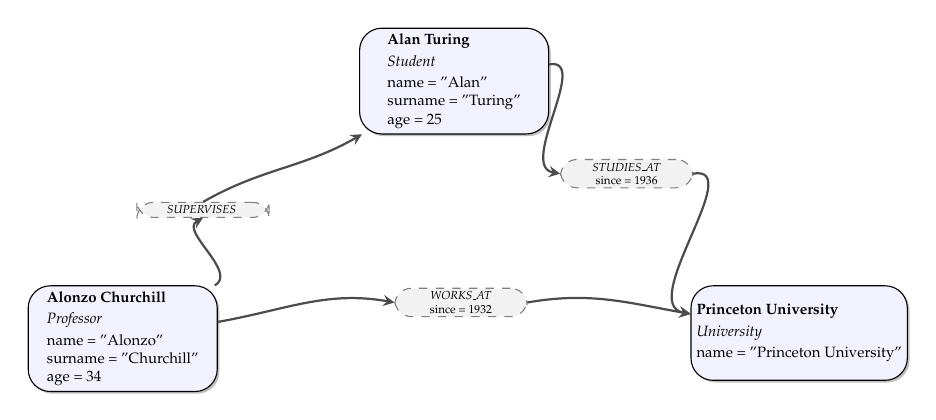
\begin{tikzpicture}[scale=0.60, transform shape,
  node/.style={
    rectangle, draw=black, rounded corners=8pt, fill=blue!5,
    minimum width=4cm, minimum height=2cm, align=left, font=\small, drop shadow
  },
  edge/.style={
    ->, >=stealth, thick, color=black!70
  },
  property/.style={
    rectangle, draw=black!50, dashed, rounded corners=6pt, fill=gray!10,
    inner sep=2pt, minimum width=2.8cm, align=center, font=\scriptsize
  },
  every shadow/.style={
    shadow xshift=0.8pt,
    shadow yshift=-0.8pt
  }
]

% Nodes
\node[node] (turing) {
  \textbf{Alan Turing} \\[2pt]
  \textit{Student} \\[2pt]
  name = "Alan" \\ 
  surname = "Turing" \\
  age = 25
};
\node[node, below left=3.2cm and 3cm of turing] (churchill) {
  \textbf{Alonzo Churchill} \\[2pt]
  \textit{Professor} \\[2pt]
  name = "Alonzo" \\ 
  surname = "Churchill" \\
  age = 34
};
\node[node, below right=3.2cm and 3cm of turing] (princeton) {
  \textbf{Princeton University} \\[2pt]
  \textit{University} \\[2pt]
  name = "Princeton University"
};

% Edge Properties
\node[property, above=0.4cm of $(turing)!0.5!(princeton)$] (studies) {
  \textit{STUDIES\_AT} \\ 
  since = 1936
};
\node[property, above=0.4cm of $(churchill)!0.5!(princeton)$] (works) {
  \textit{WORKS\_AT} \\ 
  since = 1932
};
\node[property, left=0.4cm of $(churchill)!0.5!(turing)$] (supervises) {
  \textit{SUPERVISES}
};

% Edges
\draw[edge] (turing) to[out=10,in=170] (studies.west);
\draw[edge] (studies.east) to[out=10,in=170] (princeton);

\draw[edge] (churchill) to[out=10,in=170] (works.west);
\draw[edge] (works.east) to[out=10,in=170] (princeton);

\draw[edge] (churchill) to[out=30,in=210] (supervises.south);
\draw[edge] (supervises.north) to[out=30,in=210] (turing);

\end{tikzpicture}
}
\end{center}


\end{frame}

\begin{frame}{Graph Databases}
    \uncover<1->{\textbf{What are Graph Databases?}}
    \begin{itemize}
        \item<2-> Storage systems optimized for graphs
        \item<3-> Allow to efficiently query the underlying graphs, thus using the graph as a knowledge base!
    \end{itemize}
\end{frame}


\begin{frame}{GraphDBs and AI}
\begin{center}
\begin{tikzpicture}[scale=0.70,
  box/.style={
    rectangle, draw=#1, fill=#1!20, rounded corners=5pt,
    minimum width=2.5cm, minimum height=1.5cm, thick
  },
  arrow/.style={
    ->, >=stealth, thick
  },
  example/.style={
    font=\tiny, text width=2.5cm, align=center
  }
]

% Main components
\node[box=primary] (user) at (0, 0) {User Query};
\node[example, below=0.1cm of user] {};

\node[box=nodeblue] (graphdb) at (3, 3) {GraphDB};
\node[example, above=0.1cm of graphdb] {};

\node[box=accent] (llm) at (8, 0) {LLM};

\node[box=green!70!black] (response) at (12, 0) {Response};
\node[example, below=0.1cm of response] {};

% Context box
\node[rectangle, draw=nodeblue, fill=nodeblue!10, dashed,
      minimum width=3cm, minimum height=1cm]
      (context) at (8, 3) {Domain Context};
\node[example, above=0.1cm of context] {};

% Arrows with labels
\draw[arrow] (user) -- (graphdb);
\draw[arrow] (graphdb) -- (context);
\draw[arrow] (context) -- (llm);
\draw[arrow] (user) -- (llm);
\draw[arrow] (llm) -- (response);

\end{tikzpicture}
\end{center}
\end{frame}

\begin{frame}{Our contribution}
  \centering 

  % Main title
  \uncover<1->{
  {\Large A Computation-Friendly\\Compressed Graph Database}
  }

  \vspace{0.5cm}


  \uncover<2->{
  % Diagram rewritten for a robust and adaptive layout
  \begin{tikzpicture}[
      node distance=0.25cm, % Controls spacing between components
      % Define styles for consistent and clean code
      box/.style={rounded corners, align=center, minimum height=1.7cm},
      focus/.style={box, draw=accent, fill=accent!20, text width=2.4cm, font=\bfseries},
      component/.style={box, draw=nodeblue, fill=nodeblue!20, text width=1.8cm},
      container/.style={draw=primary, fill=primary!10, rounded corners, inner sep=0.4cm}
    ]
    % Place nodes relative to each other for a flexible layout
    \node[component] (structure) {Graph Structure};
    \node[component, right=of structure] (types) {Type\\System};
    \node[component, right=of types] (props) {Properties\\Support};
    \node[component, right=of props] (query) {Query\\Engine};

    % Use the 'fit' library to draw a container around the component nodes.
    % The 'backgrounds' library draws it behind the nodes.
    \begin{pgfonlayer}{background}
      \node[container, fit=(structure) (query)] (main_box) {};
    \end{pgfonlayer}
  \end{tikzpicture}
  }

  \vspace{\stretch{1}}

  \uncover<2->{
  \begin{tcolorbox}[
    colback=accent!15,      % Light accent background color
    colframe=accent,        % Solid accent frame color
    width=\textwidth,       % Set width to the full text width
    boxrule=0.5pt,          % Thin frame rule
    arc=2mm                 % Slightly rounded corners
  ]
    It outperforms state-of-the-art GraphDBs in both time and space efficiency.
  \end{tcolorbox}
  }

  \vspace{\stretch{2}}
\end{frame}

\section{A new integer compression idea}

\begin{frame}{How graphs are represented?}
  \begin{columns}[T]
    \begin{column}{0.35\textwidth}
      \centering
      \uncover<1->{
      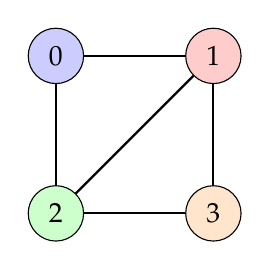
\begin{tikzpicture}[scale=1.0]
        % Draw a simple graph
        \node[circle, draw, fill=blue!20, minimum size=20pt] (0) at (0,2) {0};
        \node[circle, draw, fill=red!20, minimum size=20pt] (1) at (2,2) {1};
        \node[circle, draw, fill=green!20, minimum size=20pt] (2) at (0,0) {2};
        \node[circle, draw, fill=orange!20, minimum size=20pt] (3) at (2,0) {3};

        % Draw edges
        \draw[thick] (0) -- (1);
        \draw[thick] (0) -- (2);
        \draw[thick] (1) -- (3);
        \draw[thick] (2) -- (3);
        \draw[thick] (1) -- (2);
      \end{tikzpicture}
      }
    \end{column}

    \begin{column}{0.65\textwidth}
      \centering
      \uncover<1->{
      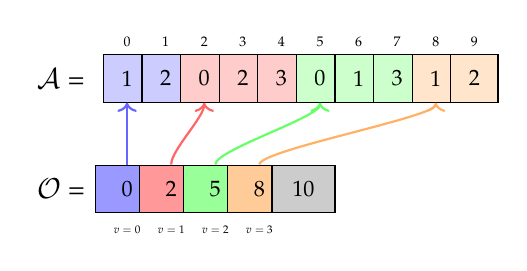
\begin{tikzpicture}[scale=0.7]
        % Array A (adjacency array)
        \node at (-1.2, 1) {$\mathcal{A}$ =};
        \foreach \x/\val/\col in {0/1/blue!20, 1/2/blue!20, 2/0/red!20, 3/2/red!20, 4/3/red!20, 5/0/green!20, 6/1/green!20, 7/3/green!20, 8/1/orange!20, 9/2/orange!20} {
          \node[rectangle, draw, fill=\col, minimum width=0.6cm, minimum height=0.6cm, font=\footnotesize] (A\x) at (\x*0.7,1) {\val};
          \node[above, font=\tiny] at (\x*0.7,1.4) {\x};
        }

        % Array O (offset array) - proper array with adjacent cells
        \node at (-1.2, -1) {$\mathcal{O}$ =};
        \foreach \x/\val/\col in {0/0/blue!40, 1/2/red!40, 2/5/green!40, 3/8/orange!40, 4/10/gray!40} {
          \node[rectangle, draw, fill=\col, minimum width=0.8cm, minimum height=0.6cm, font=\footnotesize] (O\x) at (\x*0.8,-1) {\val};
        }

        % Labels for vertices - smaller and in math mode
        \foreach \x/\v in {0/0, 1/1, 2/2, 3/3} {
          \node[below, font=\fontsize{4pt}{5pt}\selectfont] at (\x*0.8,-1.5) {$v=\v$};
        }

        % Arrows showing offset connections
        \draw[->, thick, blue!60] (O0.north) .. controls (0,-0.3) and (0,0.3) .. (A0.south);
        \draw[->, thick, red!60] (O1.north) .. controls (0.8,-0.3) and (2*0.7,0.3) .. (A2.south);
        \draw[->, thick, green!60] (O2.north) .. controls (1.6,-0.3) and (5*0.7,0.3) .. (A5.south);
        \draw[->, thick, orange!60] (O3.north) .. controls (2.4,-0.3) and (8*0.7,0.3) .. (A8.south);
      \end{tikzpicture}
      }
    \end{column}
  \end{columns}

  \vspace{0.5cm}
    \uncover<2->{
    \begin{center}
    \begin{tcolorbox}[
    colback=accent!15,      % Light accent background color
    colframe=accent,        % Solid accent frame color
    width=\textwidth,       % Set width to the full text width
    boxrule=0.5pt,          % Thin frame rule
    arc=2mm                 % Slightly rounded corners
  ]
    Compressing graphs is an integer compression problem!
  \end{tcolorbox}
    \end{center}
    }
    \vspace{0.5cm}
\end{frame}

\begin{frame}{An integer compression problem}
    \vspace{0.75cm}

    \uncover<1->{
    \begin{center}
    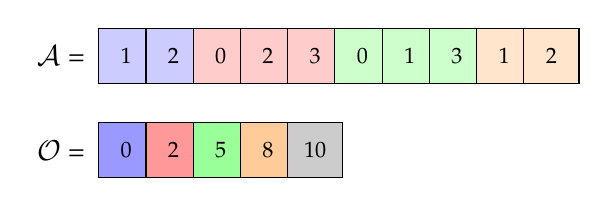
\begin{tikzpicture}[scale=0.8]
        % Array A (adjacency array)
        \node[anchor=east] at (-0.5, 1) {$\mathcal{A}$ =};
        \foreach \x/\val/\col in {0/1/blue!20, 1/2/blue!20, 2/0/red!20, 3/2/red!20, 4/3/red!20, 5/0/green!20, 6/1/green!20, 7/3/green!20, 8/1/orange!20, 9/2/orange!20} {
          \node[rectangle, draw, fill=\col, minimum width=0.7cm, minimum height=0.7cm, font=\footnotesize] (A\x) at (\x*0.75, 1) {\val};
        }

        % Array O (offset array)
        \node[anchor=east] at (-0.5, -0.5) {$\mathcal{O}$ =};
        \foreach \x/\val/\col in {0/0/blue!40, 1/2/red!40, 2/5/green!40, 3/8/orange!40, 4/10/gray!40} {
          \node[rectangle, draw, fill=\col, minimum width=0.7cm, minimum height=0.7cm, font=\footnotesize] (O\x) at (\x*0.75, -0.5) {\val};
        }
    \end{tikzpicture}
    \end{center}
    }

    \begin{itemize}
        \item<1-> $\mathcal{O}$ is monotonically increasing, thus easily compressible with existing techniques (e.g., Elias-Fano and Interpolative codes). 
        \item<2-> $\mathcal{A}$ is just locally sorted. We need \emph{something new}.
    \end{itemize}

    \vspace{2cm}
\end{frame}

\begin{frame}{A new cluster-aware integer compression technique}
\begin{center}
  \uncover<1->{
  \begin{tcolorbox}[
    colback=accent!15,      % Light accent background color
    colframe=accent,        % Solid accent frame color
    width=\textwidth,       % Set width to the full text width
    boxrule=0.5pt,          % Thin frame rule
    arc=2mm                 % Slightly rounded corners
  ]
    We generalize the problem of compressing a sequence $\mathcal S$ of \(n\) non-negative integers, knowing that \emph{consecutive integers might be monotonically increasing}.
  \end{tcolorbox}
  }

  \vspace{0.5cm}

  \uncover<2->{For example,}

  \uncover<2->{
  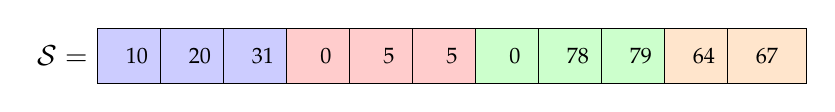
\begin{tikzpicture}[scale=0.8]
    \node[anchor=east] at (-0.5, 1) {$\mathcal{S} = \; $};
    \foreach \x/\val/\col in {0/10/blue!20, 1/20/blue!20, 2/31/blue!20, 3/0/red!20, 4/5/red!20, 5/5/red!20, 6/0/green!20, 7/78/green!20, 8/79/green!20, 9/64/orange!20, 10/67/orange!20} {
        \node[rectangle, draw, fill=\col, minimum width=1.0cm, minimum height=0.7cm, font=\footnotesize] (A\x) at (\x*1.0, 1) {\val};
    }
  \end{tikzpicture}
  }
\end{center}
\end{frame}

\begin{frame}{The intuition}
\uncover<1->{
\begin{tcolorbox}[
    colback=accent!15,      % Light accent background color
    colframe=accent,        % Solid accent frame color
    width=\textwidth,       % Set width to the full text width
    boxrule=0.5pt,          % Thin frame rule
    arc=2mm                 % Slightly rounded corners
  ]
    Consecutive elements of $\mathcal S$ often share their most significant bits.
  \end{tcolorbox}
}
  \vspace{0.5cm}

\uncover<2->{
  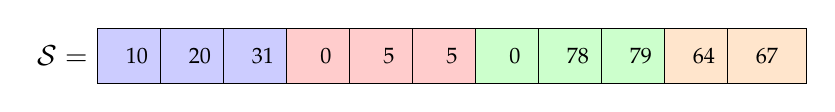
\begin{tikzpicture}[scale=0.8]
    \node[anchor=east] at (-0.5, 1) {$\mathcal{S} = \; $};
    \foreach \x/\val/\col in {0/10/blue!20, 1/20/blue!20, 2/31/blue!20, 3/0/red!20, 4/5/red!20, 5/5/red!20, 6/0/green!20, 7/78/green!20, 8/79/green!20, 9/64/orange!20, 10/67/orange!20} {
        \node[rectangle, draw, fill=\col, minimum width=1.0cm, minimum height=0.7cm, font=\footnotesize] (A\x) at (\x*1.0, 1) {\val};
    }
  \end{tikzpicture}
}

    \vspace{0.25cm}
\uncover<2->{
    \begin{center}
    \text{\tiny Binary Representation}\\[0.3cm]
    \small
    \begin{tabular}{c|c|c|c}
        \hline
        10: \textcolor{orange!70}{\textbf{000}}1010 & 0: \textcolor{red!70}{\textbf{000}}0000 & 0: \textcolor{red!70}{\textbf{000}}0000 & 64: \textcolor{green!70}{\textbf{100}}0000 \\
        20: \textcolor{blue!70}{\textbf{001}}0100 & 5: \textcolor{red!70}{\textbf{000}}0101 & 78: \textcolor{green!70}{\textbf{100}}1110 & 67: \textcolor{green!70}{\textbf{100}}0011 \\
        31: \textcolor{blue!70}{\textbf{001}}1111 & 5: \textcolor{red!70}{\textbf{000}}0101 & 79: \textcolor{green!70}{\textbf{100}}1111 & \\
    \end{tabular}

    \vspace{0.25cm}
\end{center}
}
\end{frame}

\begin{frame}{The strategy}
  \begin{tcolorbox}[
    colback=accent!15,      % Light accent background color
    colframe=accent,        % Solid accent frame color
    width=\textwidth,       % Set width to the full text width
    boxrule=0.5pt,          % Thin frame rule
    arc=2mm                 % Slightly rounded corners
  ]
  We keep a binary vector \(\mathcal{B}\) indicating whether each element's \(h\) most significant bits match those of the previous element. We store these bits only once per \emph{cluster}.
  \end{tcolorbox}
  \vspace{0.3cm}
\end{frame}

\begin{frame}{Example}
    \uncover<1->{
    \begin{tcolorbox}[
    colback=accent!15,      % Light accent background color
    colframe=accent,        % Solid accent frame color
    width=\textwidth,       % Set width to the full text width
    boxrule=0.5pt,          % Thin frame rule
    arc=2mm                 % Slightly rounded corners
    ]
    We keep a binary vector \(\mathcal{B}\) indicating whether each element's \(h\) most significant bits match those of the previous element. We store these bits only once per \emph{cluster}.
    \end{tcolorbox}
    }

    \vspace{0.05cm}

    \uncover<1->{
    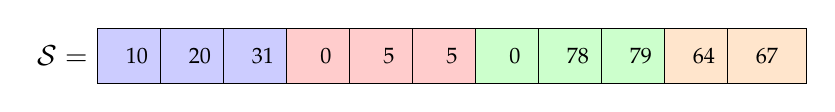
\begin{tikzpicture}[scale=0.8]
    \node[anchor=east] at (-0.5, 1) {$\mathcal{S} = \; $};
    \foreach \x/\val/\col in {0/10/blue!20, 1/20/blue!20, 2/31/blue!20, 3/0/red!20, 4/5/red!20, 5/5/red!20, 6/0/green!20, 7/78/green!20, 8/79/green!20, 9/64/orange!20, 10/67/orange!20} {
        \node[rectangle, draw, fill=\col, minimum width=1.0cm, minimum height=0.7cm, font=\footnotesize] (A\x) at (\x*1.0, 1) {\val};
    }
  \end{tikzpicture}
    }

    \vspace{-0.25cm}
    \uncover<2->{
    \text{\scriptsize With \(h=3\) we have:}
    
    \scriptsize
    \renewcommand{\arraystretch}{1.1}
    \setlength{\tabcolsep}{3pt}

    \begin{columns}[T]
    \begin{column}{0.48\textwidth}
    \begin{tabular}{c|c|c|c|c|c}
        \hline
        $i$ & $\mathcal{S}[i]$ & Binary & $\mathcal{B}[i]$ & $\mathcal{H}[i]$ & $\mathcal{L}[i]$ \\
        \hline
        0 & 10 & \textcolor{orange!70}{\textbf{000}}1010 & 1 & 000 & 1010 \\
        1 & 20 & \textcolor{blue!70}{\textbf{001}}0100 & 1 & 001 & 0100 \\
        2 & 31 & \textcolor{blue!70}{\textbf{001}}1111 & 0 & --- & 1111 \\
        3 & 0  & \textcolor{red!70}{\textbf{000}}0000 & 1 & 000 & 0000 \\
        4 & 5  & \textcolor{red!70}{\textbf{000}}0101 & 0 & --- & 0101 \\
        5 & 5  & \textcolor{red!70}{\textbf{000}}0101 & 0 & --- & 0101 \\
        6 & 0  & \textcolor{red!70}{\textbf{000}}0000 & 0 & --- & 0000 \\
        \hline
    \end{tabular}
    \end{column}

    \begin{column}{0.48\textwidth}
    \begin{tabular}{c|c|c|c|c|c}
        \hline
        $i$ & $\mathcal{S}[i]$ & Binary & $\mathcal{B}[i]$ & $\mathcal{H}[i]$ & $\mathcal{L}[i]$ \\
        \hline
        7 & 78 & \textcolor{green!70}{\textbf{100}}1110 & 1 & 100 & 1110 \\
        8 & 79 & \textcolor{green!70}{\textbf{100}}1111 & 0 & --- & 1111 \\
        9 & 64 & \textcolor{green!70}{\textbf{100}}0000 & 0 & --- & 0000 \\
        10 & 67 & \textcolor{green!70}{\textbf{100}}0011 & 0 & --- & 0011 \\
        & & & & & \\
        & & & & & \\
        & & & & & \\
        \hline
    \end{tabular}
    \end{column}
    \end{columns}
    }

    \vspace{0.05cm}
    \uncover<2->{
    \text{where $\mathcal H$ and $\mathcal L$ are the arrays storing high and low bits, respectively.}
    }
    \vspace{0.2cm}
\end{frame}

\begin{frame}{On space usage}
    \uncover<1->{
    \begin{tcolorbox}[
    colback=accent!15,      % Light accent background color
    colframe=accent,        % Solid accent frame color
    width=\textwidth,       % Set width to the full text width
    boxrule=0.5pt,          % Thin frame rule
    arc=2mm                 % Slightly rounded corners
  ]
    The overall space strongly depends on the \emph{split point} \(h\) employed.
  \end{tcolorbox}
    }

\pause % MODIFICA

\uncover<2->{
\begin{center}
  \begin{tikzpicture}[scale=0.75]
    % Axes
    \draw[->] (0,0) -- (6,0) node[right] {\scriptsize $h$};
    \draw[->] (0,0) -- (0,4) node[above] {\scriptsize \(\mathrm{Space}(\mathcal S, h)\)};

    % Curve
    \draw[thick, nodeblue] plot[smooth] coordinates {
      (0.5,3.5) (1,2.8) (1.5,2.2) (2,1.8) (2.5,1.6) (3,1.5) (3.5,1.7) (4,2.1) (4.5,2.6) (5,3.2) (5.5,3.8)
    };

    % Optimal point
    \fill[accent] (3,1.5) circle (0.1);
    \draw[dashed, accent] (3,0) -- (3,1.5);
    \node[below, accent] at (3,0) {$h^*$};
    \node[above, accent] at (3,1.7) {\scriptsize Sweet spot};
  \end{tikzpicture}
  \end{center}
  }
  \vspace{0.25cm}
\end{frame}



\begin{frame}{It's good news time}

    \visible<1->{%
    \begin{tcolorbox}[
        colback=accent!15,
        colframe=accent,
        width=\textwidth,
        boxrule=0.5pt,
        arc=2mm
    ]
    The overall space strongly depends on the \emph{split point} \(h\) employed, but we designed a linear-time algorithm to find the best the optimal one.
    \end{tcolorbox}
    }

    \vspace{0.25cm}

    \visible<2->{%
    \begin{tcolorbox}[
        colback=accent!15,
        colframe=accent,
        width=\textwidth,
        boxrule=0.5pt,
        arc=2mm
    ]
    This scheme supports \( O(1) \)-time retrieval of arbitrary elements.
    \end{tcolorbox}
    }

    \vspace{0.25cm}

    \visible<3->{%
    \begin{tcolorbox}[
        colback=accent!15,
        colframe=accent,
        width=\textwidth,
        boxrule=0.5pt,
        arc=2mm
    ]
    Our compressed graph supports adjacency queries in \( O(1) \)-time. No need to decompress the whole neighborhood/graph!
    \end{tcolorbox}
    }

\end{frame}
  

\section{Results}
% I will do this section my self

\begin{frame}{Our competitors}
    We benchmarked our Compressed Graph Database against state-of-the-art graph compressors and commercial GraphDBs on several real-world graph datasets.
\end{frame}



\begin{frame}[t]{Space: Comparison with GraphDBs}
  \begin{center}
    \includegraphics[
    width=1.0\textwidth,
    height=1.0\textheight,
    keepaspectratio
  ]{plots/graphdb_storage-1.pdf}  
  \end{center}
\end{frame}

\begin{frame}{Space: Comparison with other Graph Compressors}
\centering
    \includegraphics[
    width=1.0\textwidth,
    height=1.0\textheight,  % MODIFICA: Leggermente ridotto per un miglior margine
    keepaspectratio
  ]{plots/space.pdf}
\end{frame}

\begin{frame}{Time-space tradeoffs: GraphDBs}
% Annouce: we are up to 10x faster in neighborhood queries than commercial GraphDBs

\begin{tcolorbox}[
    colback=accent!15,      % Light accent background color
    colframe=accent,        % Solid accent frame color
    width=\textwidth,       % Set width to the full text width
    boxrule=0.5pt,          % Thin frame rule
    arc=2mm                 % Slightly rounded corners
  ]
    Our Compressed GraphDB achieves up to 10x faster neighborhood query performance compared to commercial GraphDBs.
  \end{tcolorbox}

\end{frame}

\begin{frame}{Time-space tradeoffs: other Graph Compressors}
  \centering
    \includegraphics[
    width=1.0\textwidth,
    height=0.8\textheight,  % MODIFICA: Leggermente ridotto per un miglior margine
    keepaspectratio
  ]{plots/dblp.pdf}
  
  
\end{frame}


\begin{frame}
\huge Thanks for your attention    
\end{frame}

\end{document}